% Preamble ------------------------------------------------------------------------

\documentclass[11pt]{article}

 % Package Loads ------------------------------------------------------------------

 \usepackage[utf8]{inputenc}
 \usepackage[T1]{fontenc}
 \usepackage{lmodern}

 \usepackage[letterpaper, total={6.5in, 9in}, footnotesep=0.3in]{geometry}
 \usepackage[colorlinks=true, allcolors=blue]{hyperref}
 \usepackage{sidecap, caption}
 \usepackage{enumitem}
 \usepackage{csquotes}

 \usepackage{graphicx}
 \usepackage{float}

 \usepackage{units}
 \usepackage{amsmath,amsfonts,amssymb}
 \usepackage{gensymb}
 
 \usepackage{titlesec}
 \usepackage{titling}
 \usepackage{authblk}
 \usepackage[style=numeric]{biblatex}

 % Path ---------------------------------------------------------------------------

 \graphicspath{{assets/}}
 \addbibresource{bibliography.bib}

 % Set Global Font ----------------------------------------------------------------

 \renewcommand{\rmdefault}{lmss}

 % Title Elements -----------------------------------------------------------------
 

 \title{
    {\vspace{-1.5cm}}
    {\hspace{-2cm}}   
    {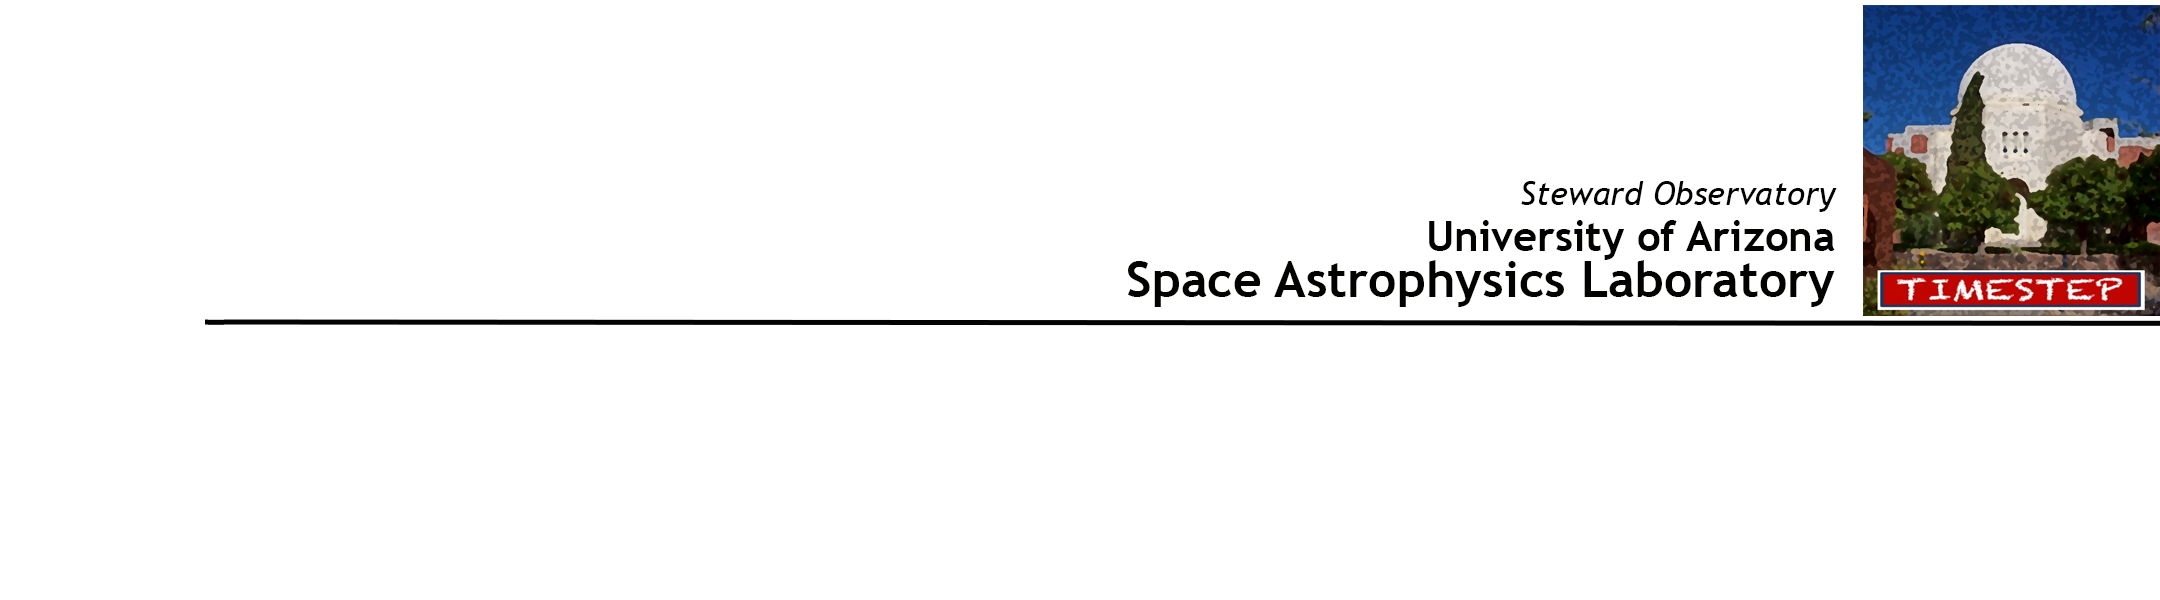
\includegraphics{TimestepHeader.png}}
    {\large Primer of}\\
    {Optical Laboratory Methods}\\
    {\Large \textit{Techniques \& Tips for Keeping your Lab Manager Happy}}
 } 

 \author{\large Jess Johnson}

 \affil{\small Senior Instrumentation Scientist \\ Steward Observatory, University of Arizona \\ November 23, 2023}

 \date{}

% Document Start ------------------------------------------------------------------

\begin{document}

\fontfamily{lmss}
\maketitle

% Abstract ------------------------------------------------------------------------

\begin{abstract}

The following short primer is an overview of what should be known before stepping foot into an optical laboratory for the first time. Optical labs run the gamut of configurations, from extreme clean room environments to small educational setups, but there are common considerations and etiquette expectations that all labs share. Most optical labs have a lab manager, who is responsible for keeping track of parts inventories, maintaining laboratory cleanliness and equipment functionality, enforcing mandated rules and regulations, and monitoring experiments. Staying on the good side of the lab manager is essential to your success in the lab. The sections in this primer will help you do just that, while simultaneously helping to assure the safety of yourself, your co-workers, and the ridiculously pricey lab equipment.

\vspace{5mm}

\textit{\textbf{Author's notes}: This primer is part one of a two part series. The second part, \textit{Working with Laboratory Optical Setups}, discusses basic elements of optical design, how to setup up an optical experiment, and optical system alignment.}

\textit{Also, this document was designed to be read with Adobe Reader (or Acrobat). The links work if using that software; they may not work with other PDF readers.}

\end{abstract}

\newpage

% Table of Contents ---------------------------------------------------------------

\tableofcontents

\newpage

% Section One ---------------------------------------------------------------------

\section{Introduction}
If you are about to enter an optics lab for the first time, you probably have a lot of questions, and most of them have probably  not been answered by the powers that be. This short primer is meant to catch you up to speed on the most important things to know before you walk through the door.

Not all optics labs are the same. They differ by purpose (optics manufacturing lab vs.~optics research lab), by their clean room type (from the European Space Agency's ISO Class 1 Microbiology Laboratory to your high school's Class 9 optics lab) and by their management level (from Pfizer Pharmaceutical's lab controllers to your high school's 8th grade physics instructor). Regardless of what particular configuration or purpose, there are ways to appropriately prepare yourself.

The following is a list of the general topics that I'll cover in more detail in the sections to follow. Consider it a roadmap: start with topic number one and work your way through the rest.

\paragraph{1. Gather Information (Section~\ref{sec:Information}):} 
Identify who is in charge of the lab. This may be a lab professor or a lab manager. Introduce yourself. Ask this person for lab rules and regulations. Ask for what training courses are required. Read up on what the lab does, or what you will be expected to do. Ask coworkers or fellow students who have worked there for inside information. 

\vspace{-10pt}

\paragraph{2. Complete Required Training (Section~\ref{sec:Training}):}
You will most likely have to complete a few training courses before working in the lab. These cover topics like laser safety, fire safety, and lab-specific safety training. 

\vspace{-10pt}

\paragraph{3. Understand Lab Etiquette (Section~\ref{sec:Etiquette}):}
There are ways to behave in laboratory settings, and most apply to all lab environments. These expectations not only help work to flow smoothly, but also help to reduce friction inbetween coworkers.

\vspace{-10pt}

\paragraph{4. Understand the Lab's Rules and Regulations (Section~\ref{sec:Rules}):}
If all went well, you should have been able to get these during the first step. Read them. Understand them. This is the key to your lab manager's heart.

\vspace{-10pt}

\paragraph{5. Understand Basic Optical Lab Techniques (Section~\ref{sec:Technique}):}
More than anything, work in an optical laboratory requires a high degree of patience and care. Very expensive things can be easily destroyed, and, as Niels Bohr was fond of saying, 'En fejl er let at lave'.

% Section Two ---------------------------------------------------------------------

\section{Gathering Information}
\label{sec:Information}

Before embarking on any new endeavor, it always pays to be as knowledgeable as possible about the situation you are about to enter into. One of the quickest ways to get up to speed is to talk to people who have experience doing whatever it is you are about to do. In the case at hand, the following are potentially helpful people to talk to. Note that not all institutions are the same. Some have lab managers, others don't. In a university student setting, there may not be a lab manager, and your instructor becomes the de facto manager. In a professional setting for production or research, there will almost always be one. Pick and choose to fit your situation.

In general, more open communication is ALWAYS better than less. When you show interest, ask valid questions, and make your intentions known, people will find it easier to communicate with you, and day-to-day interactions will be more friendly and generally smoother. With that being said, here are a few people you should practice your communications skills with.

\subsection{The Lab Manager}

From \textbf{Wikipedia}: 

"A laboratory manager (alternatively laboratory supervisor) is an individual who supervises personnel and operations in a laboratory environment; the position is senior to that of a laboratory technician or laboratory technologist, and is considered a middle-management occupation. Some laboratory managers are current or former scientists who are sometimes called "working managers," and who participate in conducting research in addition to administrative duties, mentoring students, and assisting other researchers. Managers in this category are commonly known as staff scientists."\cite{website:wikipedia01}
\vspace{0.3cm}

\hspace{-0.7cm} From \textbf{Encyclopedia Galactica}:

"Laboratory manager: noun. Someone who does precision guesswork based on unreliable data provided by those of questionable knowledge."\cite{adams}

\vspace{0.3cm}

\hspace{-0.7cm} As the lab manager is frequently called upon to interpret requests from many individuals with differing levels of communication skills, the tongue in cheek second definition is basically true, and I would add to this that lab managers frequently know more than they say and notice more than you realize. Of all the people you will encounter in a laboratory, this is the person you will most benefit from respecting, if not befriending. One look at the list of a lab manager's responsibilities should tell you why this is:

\begin{enumerate}[noitemsep]
  \item The lab manager enforces the rules of the laboratory.
  \item The lab manager enforces proper safety practices.
  \item The lab manager approves and orders equipment and supply purchases.
  \item The lab manager approves experiment designs and designates space for the experiment.
  \item The lab manager frequently reports on student/employee performance and behavior ('notice more than you realize').
  \item The lab manager is most likely a former scientist or lab technician with a wealth of knowledge ('knows more than they say').
\end{enumerate}

Seek out your lab manager before you enter the lab for the first time. Introduce yourself, explain why you will be invading... er, entering their lab. Give them your background in a few short sentences. Then ask for the following things:

\begin{itemize}[noitemsep]
  \item The rules of the lab. This can either be a printed page, a web URL, or a spoken list that you should be prepared to copy down.
  \item Which, if any, training courses are required before you begin work, and where to sign up for them.
  \item The type of clean room and what appropriate dress is.
  \item Whether there is a place to keep personal items while working.
  \item Lab access information... passwords, door codes, etc.
  \item Emergency contact numbers... who to call in case something burns down, falls over, or blows up.
  \item What irks him/her the most, specifically so that you can avoid doing it.
\end{itemize}

I can't emphasize this enough: the lab manager is someone with whom you want to have a good working relationship. They can answer technical questions about equipment, make recommendations about appropriate equipment, assist you with your experimental design, and in general, make your life much easier.

\subsection{Your Boss, Professor, or Instructor}

Whereas your lab manager can make your day-to-day existance easier in a number of different ways, the person who was responsible for your placement in the lab is, in the end, the person you have to perform \textit{for}. To this end, understanding their expectations is extremely important. So before your adventure begins, here are a few things to find out at the very start.

\begin{itemize}[noitemsep]
  \item Make sure that you clearly understand the project and the goals. If you are NOT clear on this, ask for explanation at the very start. Also, make sure you know time scales: when should the project be finished? What kind of flexibility is there in the case of unexpected delays?
  \item Find out what reporting expectations are. How frequently does she want to be updated? In what kind of format? Weekly meetings? Lab reports? Preliminary memos?
  \item Will you be expected to keep a professional lab notebook? What format? If the work you are doing is proprietary, there are most likely existing formats and requirements.
  \item Discuss time-in-the lab expectations, or if there are preferred times for you to work.
  \item Discuss the budget for ordering parts, and who approves your part orders.
\end{itemize}

In most cases, your contact with this person after your work begins will be limited. If they have minimal reporting requirements, now is a good time to ask for and set up regular meeting times. It is best to not make them seek out you for updates, so deal with this now. Ask to establish weekly or bi-weekly meetings. Take advantage of this time: be prepared to review your progress, ask for suggestions and criticism, and sketch out ideas for future work. Trying to get meeting time that has not been pre-established can be difficult.

\subsection{Previous Students or Employees}

If you know of others who have worked in the lab, or with your boss/professor/instructor, ask them to fill you in on what their experience was like. Remember, however, that everyone has an opinion, and you are more concerned here about facts. Sort out observations from attitude. 

Reasonable questions include:

\begin{itemize}[noitemsep]
  \item What is the working environment like? Do people keep to themselves, or are they approachable? 
  \item Who is a good, knowledgeable person to ask questions when the lab manager is not available? 
  \item Are lab working times strictly enforced, or is there flexibility? This goes to how carefully you have to plan steps of an experiment that could consume large amounts of time. Most labs do not have strict operating hours, but building access may be an issue if you have to leave and come back. There is nothing worse in this setting than to run out to your car to get something, only to find yourself locked out of the lab at 2am with an experiment in process.
  \item Did they enjoy working there? Why or why not?
\end{itemize}

This is not a complete list, of course, and the only guideline is you should be looking for usable information. 'The lab manager is an ogre' is not useful information. What caused the person to say that may well be. Be tactful in your approach and neutral in your response.

% Section Three -------------------------------------------------------------------

\section{Required Training}
\label{sec:Training}

Laboratories are inherently unsafe places to the untrained or uninformed individual. For certain kinds of laboratories, the dangers are obvious... harmful chemicals, ovens, burners and dangerous gases in a chemistry lab; needles, drugs, caged animals, biological contaminants in a biology lab. Although more subtle, dangers exist in all kinds of labs, with an optical lab being no exception. From high-voltage equipment to lasers with visible or invisible beams and frequent operation in the dark, optical labs pose their share of potential injury risks.

\subsection{Lab Training at UA}

The purpose of laboratory training is to minimize the risk of injury by ensuring that an employee has the training, support, equipment and information required to work safely.

At the University of Arizona, there are basically three safety courses that you can be required to take. These are:

\begin{itemize}[noitemsep]
  \item Fire Safety; 
  \item Chemical Safety; 
  \item Laser Safety.
\end{itemize}

If you are following this primer, you will have already asked which required courses you will have to complete. All required courses of this nature are online, and generally take 45-60 minutes each to complete. Information can be found here: \href{https://www.optics.arizona.edu/osc-students/lab-safety-training}{Safety Training}. Complete these courses before entering the lab.

\subsection{Lasers}

Although the content of all of these courses is important, I would suggest you pay very close attention to the course on laser safety. Lasers pose the number one risk to safety in optics laboratories, and, unless you've worked with lasers before, there is quite a lot to learn, and not all of it is intuitive. 

Most individuals just starting off in the world of optics have grown up in the age of 'safe' lasers... laser pointers, laser light shows, even kitty toys... but the lasers in optics labs are by no means safe. One of the useful things about lasers is that their beams, unlike, say, a flashlight, remains in a tight beam and does not diverge significantly. This means that the hazard from a laser is the same close to its source as it is from a distance away. And when that beam enters your eye, it is focused by the eye's lens down to a small spot on your retina, which can leave a burn or a permanent blind spot. This damage to your vision can occur instantly... as soon as the light enters your eyes. 

\vspace{.5cm}

\hspace{-0.6cm}Here are a few of the most important laser safety guidelines, in no particular order:

\begin{itemize}[noitemsep]
  \item Laser beams can be very difficult to see, especially with ambient light. Always be aware of where the path of the laser bream travels.
  \item Place a sign (can be handwritten) in an obvious place (taped to the clean room wall) that says 'Laser ON'.
  \item Wear eye protection while adjusting or aligning your setup.
  \item Turn the laser off when making major changes to your setup.
  \item Never look into the path of a laser, even with eye protection. This may seem obvious, but when aligning optics, this is an easy mistake to make.
  \item When setting up an experiment using lasers as a light source, keep the beam path higher or lower than where a person's eyes would be if they were sitting or standing.
  \item Do not place any reflective material near the beam path (except intentionally placed mirrors that are part of the experiment). Be careful while adjusting mirrored devices while the laser is on.
  \item Do not attempt to circumvent device interlocks or modify power supplies or plugs. They exist for valid safety reasons.

\end{itemize}

% Section Four -------------------------------------------------------------------

\section{Lab Etiquette}
\label{sec:Etiquette}

Ahh, etiquette... that set of unspoken rules that governs high society luncheonettes, black tie operas, and... laboratories?

Although one may not make the connection, etiquette is simply a set of guidelines for interacting with other humans, and unless you are on night shift in the lab, you will be working with other humans. And some humans just have difficulties interacting with others. The stereotype of an impolite labmate is so common that Nature magazine wrote about it in 2017: \href{https://www.nature.com/articles/nj7664-481a}{Nature Article}.

Whereas the particular rules of the laboratory you are working in may differ, they are at least usually written out and available. Etiquette is the set of unwritten rules that are just as important, if not more so, because they are an attempt to make person-to-person interactions courteous and respectful. And, beyond just being annoying, poor laboratory etiquette can lead to unsafe work environments and ruined experiments.
\vspace{.5cm}

\hspace{-0.6cm}Here, then, is a list of guidelines for proper laboratory etiquette.

\begin{enumerate}[noitemsep]
  \item If you borrow something, return it to whom or wherever you borrowed it from \textit{as soon as you are finished with it}.
  \item Clean up after yourself. Return the space you are using to the shape it was in when you started.
  \item Corollary: if the space needs to be organized/cleaned to start with, do it.
  \item Don't hoard shared equipment.
  \item Don't 'borrow' other peoples things, no matter how small. A missing pen can drive someone nuts.
  \item Be aware of your volume level. Respect those that need a quiet environment to think. 
  \item Assist with common tasks. If the garbage can is filled, don't stack your trash in a heap on top of it. Empty the trash can.
  \item If you see replaceable supplies running low, alert the lab manager. Nothing is more infuriating then not being able to work because there is only one left-handed glove left.
  \item Don't hide mistakes. If you break something, it happens. By letting the lab manager know, it can be promptly replaced.
  \item Perhaps the most important rule: treat everyone with the respect that you yourself would like to be shown.

\end{enumerate}

% Section Five --------------------------------------------------------------------

\section{Rules and Regulations}
\label{sec:Rules}

Although all laboratories will have their own set of rules and regulations that are informed by the purpose of the particular lab, there is a common set of basic rules that is applicable to most laboratory settings.

\subsection{Standard Laboratory Rules}

The following are reprinted from 'Ten Safety Rules Every Researcher Should Follow':\cite{website:Majumder20}. I removed a long rule that only applies exclusively to chemistry labs. Remember, these are \textit{general} rules meant to apply to all laboratory  settings; but they all are adaptable to optical settings.

\begin{enumerate}[noitemsep]
  \item \textbf{Wear protective lab attire}: Make sure you use PPE (Personal Protective Equipment) at all times inside the laboratory. Put on a lab coat with full sleeves, closed-toe shoes, and safety goggles before entering the lab. If you have long hair, it’s better to keep it tied and out of the way when working in the lab. Find out if the work you are currently doing needs you to wear any other protective gear or remove accessories such as metal watches, rings, etc. Protective attire not only reduces the risk of damage to the skin and eyes, but also minimizes possibilities of contamination.
  \item \textbf{Do not bring food or drink into the lab}: It may be tempting to sip on a cup of coffee or some water when working at your experiments, but steer clear of this. Food and drink in the lab can not only get messy, but can also be a source of distraction. Moreover, there is a possibility of contamination as chemical residues may be present on tables and on your hand when you are working in the lab. Also, make sure you wash your hands well before leaving the lab. Traces of harmful chemicals, tissue, bacteria, etc. can lead to contamination of other spaces such as the lunch table or your work station, causing illness or other problems.
  \item \textbf{Dispose of lab waste safely}: This is one area of lab safety that researchers often tend to neglect. When disposing chemicals, do not pour them down the sink; use designated disposal bins or containers instead. Never pour back unused reagents into the bottle; dispose of them safely. Do not pour plant waste down the sink as it may clog up the drains; make sure you use disposal bins to dispose plant waste.
  \item \textbf{Handle lab equipment carefully}: Apart from chemicals, laboratory equipment can also cause accidents if mishandled. Use razor blades with caution, unplug hot plates, and switch off Bunsen burners. If you see any electrical cords that are frayed or damaged, do not touch them and report it to the relevant authorities immediately. Handle broken glassware carefully; do not use your hands to pick up the pieces – a broom and dustpan work best. Remember to put back all equipment in its proper place after use.
  \item \textbf{Know what to do in case of fire}: Always store inflammable material in fireproof cabinets. Make sure you put them back in their designated cabinets after use; it’s extremely dangerous to leave them lying around. Use Bunsen burners and hot surfaces with caution. Always follow instructions when producing substances that have explosive properties. Find out the location of the fire extinguisher as soon as you start working in a lab. While you should definitely use the fire extinguisher as a first step, in case you see the fire spreading or the extinguisher not having the desired effect, call the fire department immediately.
  \item \textbf{Restrict your experiments to the lab}: Do not carry lab equipment home or to any other place for preparation or any other purpose. This could lead to contamination of the experiment as well as the other environment. It’s best to wash the clothes you’ve used in the lab before reusing them.
  \item \textbf{Do not panic in case of accidents}: Even after taking precautions, accidents do happen. In case of an accident, don’t panic. Panic can worsen the situation. Stay calm; don’t run as you might trip over wires or knock down chemical bottles. It’s important to know the location of safety equipment, such as the fire extinguisher, first aid kit, emergency phone, eyewash stations, etc. If chemicals or particles get into your eyes or skin, wash them off immediately. Take lab safety drills seriously; attending these regularly will prepare you for actual emergencies. Finally, always keep your supervisor informed about your experiment and follow their instructions carefully.
  \item \textbf{Work with a lab partner as far as possible}: Try to work with someone else in the lab. While this may not always be possible, having a second pair of eyes increases chances of mistakes and slip-ups getting detected on time, preventing major damage. Additionally, with two people, response is always quicker in case of accidents. Even for a minor injury, like a cut from broken glass, it helps to have someone around to get the first aid kit or help with cleaning the glass.
  \item \textbf{Act responsibly in the lab}: While the lab is meant for experiments, they should be planned and researched well in advance. Don’t conduct random experiments just for fun. You should have the right attitude when you come to the lab and make sure you’re fully focused. A little distraction can often cause irreversible damage, and in extreme situations, even loss of lives. Alert others in the lab to maintain a safe distance when mixing chemicals or dealing with potentially hazardous substances. Make sure you double-check everything before use and clean up after.
\end{enumerate}

\subsection{Clean Room Attire \& Gowning}

To elaborate on point number one above, if the lab you are working in is a clean room environment, you will be expected to prepare yourself through a process called 'gowning'. If this is unfamiliar, read on.

\subsubsection{What is a Clean Room?}

A Clean Room (or 'Cleanroom' in the biological sciences) is a room which regulates the amount of particles in its air according to established standards. The International Organization for Standards (ISO) is an international body which determines accepted values across a range of industrial and scientific processes. 

According to ISO 14644-1 Clause 2.1.1, \cite{website:ISO99}, a clean room is:

\begin{displayquote}
    "A room in which the concentration of airborne particles is controlled, and which is constructed and used in a manner to minimize the introduction, generation, and retention of particles inside the room and in which other relevant parameters, such as temperature, humidity and pressure are controlled as necessary." 
\end{displayquote}

Because such fanatical attention is payed to the purity of the air, you might imagine that there would be a procedure to prepare to enter a clean room, and you'd be right. It's called 'gowning'.

\subsubsection{Gowning}

Entering a clean room requires that one removes accoutrement and as much unessential clothing as is possible and cover what is left. Depending on the size and type of clean room, there may be a room in which this is done, called the \textit{anteroom}.

The anteroom provides an air-lock to the clean room itself. This is where cleaning supplies, gowning supplies, and usually a rack for personal possessions are all kept. One enters the anteroom and closes the entrance door, and then goes through the gowning procedure. When this is finished, the clean room itself can be safely entered through the second door, which is then closed.

In clean room setups that do not have an anteroom, the rest of the lab acts as the de facto anteroom, and the gowning procedure occurs wherever the supplies are located.

Figure~\ref{fig:gowning} displays a fairly common gowning routine, taken from PAC's clean room website. The website is an excellent overview of clean rooms in general and all associated procedures.~\cite{website:PAC}

\begin{figure}[!b]
    \centering
    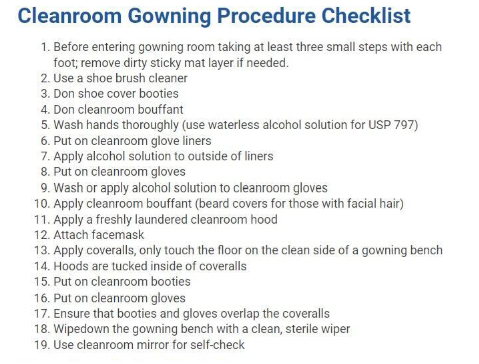
\includegraphics[height=3in]{Procedure01.png}
    \caption{The complete ISO Gowning Procedure. Not all steps apply to every laboratory.}
    \label{fig:gowning}
\end{figure}

\subsubsection{Electrostatic Protection}

In labs that deal with extremely sensitive electronics devices (deformable mirrors, CCDs), protection must be used against Electrostatic Discharge (ESD). A common ESD experience is walking across a carpet and touching a metal door handle. The spark that jumps from your finger to the handle can easily be in excess of 5,000 V, more than enough to damage electronic equipment. To prevent against this kind of thing from happening in the clean room, the gown in the above instructions is replaced by a electrostatic resistant coat and an anti-static wristband is used. The wristband is connected to a grounding strap within the clean room, providing a ground for ESD discharge. 

On the bench in a clean room is a small box called a \textit{ground mount} which is connected to a cable that runs around the bench. This provides the ground to the wristband; when you are in position to work, clamp the wristband cable to this strap. If you need to move, remove the clamp, relocate and clamp to the cable again. To check your ground (i.e., to check that the wristband is contacting your skin), plug the wriststrap clamp into the jack on the front of the ground mount when you first approach the bench.

Another thing to be aware of is that you will see anti-static table mats at locations on the bench. These are large, usually blue polymer mats that are connected, through the bench strap, to ground. These are reserved for equipment that requires safeguarding against ESD. Point of Style: lab managers get grumpy when these mats are used to store things on that do not require ESD protection.

% Section Six --------------------------------------------------------------------

\section{Optical Lab Techniques}
\label{sec:Technique}

Everything to this point has been decidedly general and non-optical in nature, and now we move to specific techniques for working in an \textit{optical} lab. These techniques are concerned with topics such as how to handle optical elements, how to store them, and the like.

This section is where this primer earns its subtitle, as everything here is the realm in which the lab manager is most intimately involved. They will expect you to \textit{at least} know and use these techniques whenever you work with optical elements and equipment. After a while, these will be burned into your muscle memory; but pay careful attention in the beginning, as not following these procedures can easily result in the destruction of very expensive objects. 

As preparation for working in the laboratory, I jokingly suggest that a new employee or student spend a few minutes looking through and optical catalog. It's an eye-opening experience, and quite motivating.

\subsection{A Small Glossary of Optical Terms}

All disciplines have their jargon, and optics is, of course, no exception. The following are a few helpful terms you'll hear in the lab.

\paragraph{Catoptric:}An optical system using reflective surfaces only.
\vspace{-10pt}
\paragraph{Catadioptric:}
An optical system that uses both reflective and refractive surfaces.
\vspace{-10pt}
\paragraph{Clear Aperture:} The actual surface area of the lens through which light can pass. For example, a 25mm lens in a mount will lose about 2mm of its diameter to the 1mm lip of the mount, leaving a 23mm diameter clear aperture.
\vspace{-10pt}
\paragraph{Collimation:}
The process of removing convergence or divergence from a light beam. On the lab bench this is usually accomplished through the use of a \textit{shear plate}.
\vspace{-10pt}
\paragraph{Eyepiece:} A lens or optical system designed to produce a virtual image for viewing by the eye or another optical system.
\vspace{-10pt}
\paragraph{Filter:} A device designed to alter either the intensity (Neutral Density filter) or spectral contents (High or Low Pass filter) of a light beam.
\vspace{-10pt}
\paragraph{Light, Coherent:}
Light whose constituent electromagnetic waves maintain a fixed and predictable phase relationship with each other. Laser light is an example of coherent light.
\vspace{-10pt}
\paragraph{Light, Incoherent:} Light whose constituent electromagnetic waves exhibit a random and unpredictable phase relationship to each. 
\vspace{-10pt}
\paragraph{Light, Monochromatic:}
Light composed of all of the same wavelength, or of a very narrow range of wavelengths, of component electromagnetic waves.
\vspace{-10pt}
\paragraph{Light, Polychromatic:}
Light composed of differing wavelength of component electromagnetic waves. White light is polychromatic.
\vspace{-10pt}
\paragraph{Mirror, Flat:}
A precision reflective optic with no curvature. Also called simply a \textit{flat}.
\vspace{-10pt}
\paragraph{Mirror, Off-Axis Parabolic:}
A precision reflective optic with a surface figure that is the off-axis portion of a paraboloid. Can be used for both collimation and focusing.
\vspace{-10pt}
\paragraph{Mount:}
A device used to hold an optical element in place.
\vspace{-10pt}
\paragraph{Objective:} A lens or optical system designed to produce a real image of a real object.
\vspace{-10pt}
\paragraph{Optic, Active:}
An optical element which uses the application of external energy to alter its optical characteristic. Liquid crystal optics will often be controlled this way.
\vspace{-10pt}
\paragraph{Optic, Compound:}
An optical component such as a compound lens or compound prism that is formed of more than one optical element. 35mm camera lenses are compound optics.
\vspace{-10pt}
\paragraph{Optic, Passive:} An optical element in which the optical characteristics of the material used is not altered by the application of external energy. Most typical laboratory optics, like lenses and prisms, are passive optics.
\vspace{-10pt}
\paragraph{Optic, Simple:} 
A single lens or prism. Also called a \textit{Singlet}.
\vspace{-10pt}
\paragraph{Optical Component:}
An optic consisting of multiple optical elements, such as beamsplitters or complex compound lens systems, and other non-lens optics, such as waveplates and pelicles. 
\vspace{-10pt}
\paragraph{Optical Device:} 
A more complex optic that typically involves an external control system, such as a deformable mirror or CCD.
\vspace{-10pt}
\paragraph{Optical Element:} 
One of the fundamental building blocks from which optical systems are designed, such as lenses, flat mirrors and prisms. Generally, only passive devices are considered optical elements. Active optics require external control systems and are typically referred to as \textit{optical devices}.
\vspace{-10pt}
\paragraph{Prescription:} The precise mathematical description of the surface figure of an optical element.
\vspace{-10pt}
\paragraph{Shear Plate:} 
An optical component that is used to test the collimation of a beam.
\vspace{-10pt}
\paragraph{Source:} 
The optical device that provides light for an optical setup. 
\vspace{-10pt}
\paragraph{Surface Figure:} Literally the shape of the optical surface of an element that controls how the element refracts or reflects light.

\subsection{Optical Laboratory Techniques}

With the glossary out of the way, we can now talk about common laboratory optical techniques. The most fundamental, and important, are listed here. You will learn many more; pay attention to your lab manager, who undoubtedly has an encyclopedic knowledge of them. 

\subsubsection{Handling Optical Elements}

Perhaps the most important set of techniques in this list. The justification for all of this is expressed extremely well in the Thorlabs tutorial on Optics Handling and Care:\cite{website:ThorLabs}

\begin{displayquote}
    "The delicate nature of optical components requires that special procedures be followed in order to maximize their performance and lifetime. Through everyday use, optics can come in contact with contaminants such as dust, water, and skin oils. These contaminants increase scatter off the optical surface and absorb incident radiation, which can create hot spots on the optical surface, resulting in permanent damage. Optical components with coatings are particularly susceptible to this sort of damage."\cite{website:ThorLabs}
\end{displayquote}

\hspace{-0.6cm}That being said, here are the procedures for handling optical components:

\begin{enumerate}[noitemsep]
   \item \textbf{Always wear gloves:} This protects the element from skin oils, which can damage the coating or surface. Removing fingerprints can risk damaging the optic.
   \item \textbf{Don't contaminate your gloves:} The purpose of the glove is to avoid transferring finger oil to the lens; however, if the glove's surface has dirt or other contaminants on it, this can be transferred as well. Replace the dirty glove, or gloves. 
   \item \textbf{Handle elements by their edges:} This keeps your fingers away from the optical surface of the element.
\end{enumerate}

\subsubsection{Unpacking Optical Elements}

You've just received a box of lenses from Newport! After grabbing the Photon Food box and hoping no one noticed, you now have to unpack your optical stuff.

\begin{enumerate}[noitemsep]
   \item \textbf{Always unpack an optical element in a clean environment:} No matter how great the temptation, don't unpack elements in your office. Take them to the clean room to unpack; this avoids dust, fingerprints, and the possibility of dropping it on a dirty floor.
   \item \textbf{Always keep the storage box:} Not the cardboard outer box, but the (usually hinged plastic) inner box that has a liner that is specifically designed to fit the element. This is not just the shipping box, but is intended to also be the storage box. It will be labelled with the description of the lens, and if the lens is always returned to its box, the next user will not have to characterize the lens (determine the focal length) before using it.
\end{enumerate}

\subsubsection{Storing Optical Elements}

For our purposes here, \textit{storing} refers to the handling of an optical element if it is not in a mount on your bench.

\begin{enumerate}[noitemsep]
   \item \textbf{Never lay an unprotected optical element on a surface.:} If you need to lay a lens down in the process of mounting or unmounting it, place a few pieces of lens tissue on the surface first. Better yet, gently wrap the lens in lens tissue and then lay it down.
   \item \textbf{Store a lens in the container it was shipped in:} For storage when not in use, wrap the lens in lens tissue and place it in its storage box, then return the storage box to the lens collection. Note that some singlets come in multi lens storage boxes; always wrap the lens in lens tissue before returning it to the box. Be sure to return the lens to its proper box, or its proper place in a multi-lens box, so that you don't have to determine the focal length before you can use it.
\end{enumerate}

\subsubsection{Mounting Optical Elements}

There are a few simple things to explain before discussing procedure. The following are useful things to know:

\begin{enumerate}[noitemsep]
   \item \textbf{Lens Sizes:} \textit{Lens Size} refers to the diameter of the lens, or other optical component. Although lenses and other components can be purchased in virtually any size diameter, there are three standardized sizes: 12.5 mm $(\frac{1}{2}")$, 25.0 mm $(1")$, and 50mm $(2")$. The most commonly used size is 1".
   \item \textbf{Mount Sizes:} Mounts are easily available in these standardized sizes. If you are using lenses in non-standard sizes, you will have to specifically order a mount that fits it.
   \item \textbf{Lens Thickness:} Lenses have two thickness measurements: \textit{Center Thickness} and \textit{Edge Thickness}. Usually, for mounting purposes, the edge thickness is the important number. If you are purchasing or using an unusually thick lens, the mount you use must be selected to be able to fit a lens of its edge thickness.
\end{enumerate}

\hspace{-0.6cm}All of the above information can be found in the supplier's part's catalog. Figure~\ref{fig:CatPage} shows a portion of a ThorLabs catalog page for Anti-Reflective Coating UV Fused Silica Plano-Convex Lenses.

\begin{figure}[!b]
    \centering
    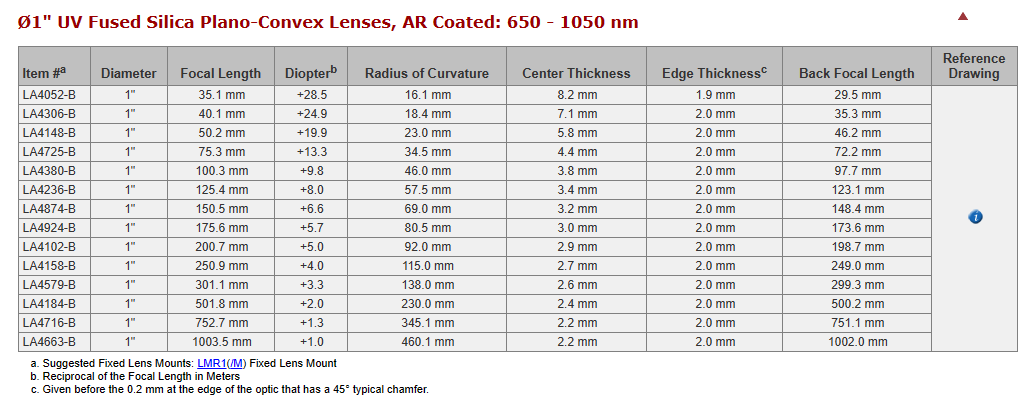
\includegraphics[height=2.5in]{assets/CatPage01.png}
    \caption{A sample page from the ThorLabs catalog, showing the typically available lens specifications.}
    \label{fig:CatPage}
\end{figure}

Given that you have your lens, or other optical component you now have to decide how you want to mount it, and what kind of mount to use. There are basically two ways to mount an optical component: Bonding and Clamping. As bonding is a relatively permanent option, most of the time you'll be using the second option, clamping. (For a discussion on bonding, as well as a complete discourse on both methods, see Jim Burge's 'Mounting of Optical Components' \cite{website:Burge01}, and 'Mounting of Lenses' \cite{website:Burge02}).

The following are the basic mount types. These are all illustrated on the following ThorLabs webpage: \href{https://www.thorlabs.com/navigation.cfm?guide_id=2307}{Mount Types}.

\vspace{10pt}

\begin{enumerate}[noitemsep]
   \item \textbf{Fixed Mount:} The most commonly used mount for singlets, filters, etc. For situations where the component doesn't need to be adjusted from side to side, forward or backward, or rotated while mounted. 
   \item \textbf{Rotation Mount:} Allows the component to be rotated. Frequently used with polarizers and components that have rotational asymmetry.
   \item \textbf{Translation Mounts:} Allows the component to move from side to side, backwards and forwards, or both. Sometimes combined with rotation, giving adjustment in all degrees of freedom.
   \item \textbf{Component Mounts:} For larger and non-standard lens sizes.
   \item \textbf{Mirror Mounts:} For flat and curved surface mirrors. Has adjusters for side-to-side tilting, top-to-bottom tipping, and rotation for curved surface mirrors
\end{enumerate}

Regardless of the type of mount the lens is clamped in basically one of two ways: tube mounting, or V-Mounting.

\paragraph{\textbf{Tube Mounting an Optical Component:}} Most optical mounts are tube mounts, as they are essentially short cylinders with a retaining lip at one end and screw threads lining the inside. The lens is placed inside the tube, resting against the lip, and then a retaining ring is threaded into the cylinder and screwed downward until it contacts the edge of the lens. There are a couple things to know.

\begin{itemize}[noitemsep]
    \item To put the lens into the mount, stick one gloved finger through the side of the mount with the lip, and then place the lens into the tube. Slowly lower your (other gloved) finger while gently pushing down on the lens until it rests on the lip. 
    \item Be extremely careful not to angle the lens such that it gets cocked and jammed against the threads. If it does, gently press on an edge to try to dislodge the lens by rotating it slightly and walking it backwards. Do not force the lens; if you can't easily remove it, this is lab manager territory.
    \item Once the lens is resting on the lip, slowly thread the retaining ring, being careful not to cross thread it. If you feel the ring tighten and not move freely, it's probably cross threaded. Back it off and re-thread it.
    \item Now, using a retaining ring spanner, gently screw the retaining ring down until it contacts the component's perimeter surface. Then gently give it a bit more force, but don't overdo it or you can crack the lens. The component is now mounted.
    \item Visually inspect the lens and mount to make sure that the lens is mounted correctly, and not tilted in the tube.
\end{itemize}

\paragraph{\textbf{V-Mounting an Optical Component:}} For large and unusually sized components (large lenses, cameras, sources, etc.), the guillotine like V-Mount is commonly used. This is basically two vertical bars, with a fixed bar at the bottom that has a V shaped notch, and a movable upper bar that has a screw in the center. This is used as follows:

\begin{itemize}[noitemsep]
    \item unscrew the side screws on the sides of the upper bar and open the mount until it is larger than the diameter of the component to be mounted.
    \item Fully retract the top bar center screw.
    \item Place the component into the V shaped notch and hold it upright.
    \item Lower the top bar until the contact surface of the center screw is about 1/4" above the edge of the lens. Tighten the side screws.
    \item The lower bar has a notch that runs along its length on the side that faces the lens, inside the V notch. If you are mounting a lens, the lens should be resting in this notch when the top screw is tightened. The contact surface of the top screw also has a notch which should be aligned with the edge of the lens.
    \item When everything is in place, screw down the top screw until it firmly holds the lens in place. Again, do not put excessive force on the lens, but assure that it is tight enough that the lens doesn't move. The lens is now mounted. Inspect it to make sure it is aligned correctly and not tilted or tipped.
    \item Larger components, like a camera, rely on the thickness of the bottom bar to hold it in place against motion, and the notch on the lower bar and upper screw don't play a role.
\end{itemize}

\subsubsection{Inspecting Optical Elements}

We have now arrived at the last of the procedures required in an optical lab, and perhaps the most fraught. Cleaning optical elements is, at best, a nerve wracking process, which is one of the reasons that so much emphasis is placed on correct handling and storing. Basically, if you can keep an element clean, there is no reason to have to clean it frequently. But even with the best of procedure, the time will come.

Because cleaning optical elements can be a destructive process unless one is well trained in the procedures, for now my advice is to take the element to your lab manager to have it cleaned. So for now, I'll present the technique for inspecting an element to determine whether it needs cleaning.

\paragraph{Inspection:}

\begin{displayquote}
"In general, optics should be inspected prior to use and before and after cleaning. It is often necessary to use a magnification device when inspecting an optical component due to the small size of most contaminants and surface defects. Even with a magnification device, it is sometimes useful to shine a bright light onto the optical surface in order to increase the intensity of the specular reflections from surface contaminants and defects.

When inspecting a reflectively coated surface, the optic should be held nearly parallel to your line of sight. By looking across the surface rather than directly at it, you will see contamination and not reflections. Polished surfaces such as lenses should be held perpendicular to your line of sight so that you can look through the optic."\cite{website:ThorLabs}
\end{displayquote}

If you notice an accumulation of dust, the presence of finger oil, or surface defects (scratches, gouges, etc.), it is time to take the element to your lab manager for cleaning or replacement.






% Section Seven --------------------------------------------------------------------

\section{Final Thoughts}

This brings us to the end of this primer. This collection of information is only an introduction; you will learn far more by watching knowledgeable individuals and asking questions then you will by committing everything discussed here to memory. But the intention is that this gets you off to a good start, and helps you avoid making common mistakes that could end up getting you on the wrong side of both your own progress, and, importantly, your lab manager.

Cheers, and good luck!

% Bibliography --------------------------------------------------------------------

\newpage

% Bibliography --------------------------------------------------------------------

\printbibliography

\end{document}
